\chapter{Monte Carlo Synthetic Acceleration\\ Methods for the
  Navier-Stokes\\ Equations\ }
\label{ch:nonlinear_problem}

In this chapter the fundamentals of Newton's method will be presented
along with a brief discussion of inexact Newton methods. Newton-Krylov
methods, a variant of inexact Newton methods, will be outlined
including an automated technique for generating the Jacobian commonly
used in today's applications. Following this, a new nonlinear solution
algorithm utilizing Monte Carlo Synthetic Acceleration will be
presented and implementation details will be discussed. Using the new
algorithm and a production fluid physics code, a group of challenging
benchmark problems for the Navier-Stokes equations will be used to
verify the correctness of the method relative to solutions obtained
using conventional methods in various flow regimes and
geometries. Finally, we will compare the performance of the new method
against contemporary Newton-Krylov methods for the same benchmark
problems.

%%---------------------------------------------------------------------------%%
\section{Preliminaries\ }
\label{sec:nonlinear_preliminaries}
We formulate the \textit{nonlinear problem} as follows
\cite{knoll_jacobian-free_2004}:
\begin{equation}
  \ve{F}(\ve{u}) = \ve{0}\:,
  \label{eq:nonlinear_problem}
\end{equation}
where $\ve{u} \in \mathbb{R}^n$ is the solution vector and
$\ve{F}:\mathbb{R}^N \rightarrow \mathbb{R}^N$ is the function of
nonlinear residuals. We write the nonlinear system in this form so
that when an exact solution for $\ve{u}$ is achieved, all residuals
evaluate to zero. \textit{Newton's method} is a root finding algorithm
and therefore we can use it to solve Eq~(\ref{eq:nonlinear_problem})
if we interpret the exact solution $\ve{u}$ to be the roots of
$\ve{F}(\ve{u})$. Newton's method is also an iterative scheme, and we
can generate this procedure by building the Taylor expansion of the
$k+1$ iterate, $\ve{F}(\ve{u}^k)$, of the nonlinear residuals about
the previous $k$ iterate, $\ve{F}(\ve{u}^{k+1})$:
\begin{equation}
  \ve{F}(\ve{u}^{k+1}) = \ve{F}(\ve{u}^{k}) +
  \ve{F}'(\ve{u}^{k})(\ve{u}^{k+1}-\ve{u}^{k}) +
  \frac{\ve{F}''(\ve{u}^{k})}{2}(\ve{u}^{k+1}-\ve{u}^{k})^2 + \cdots
  \:.
  \label{eq:newton_derivation_1}
\end{equation}
If we ignore the nonlinear terms in the expansion and assert that at
the $k+1$ iterate $\ve{u}^{k+1}$ is the exact solution such that
$\ve{F}(\ve{u}^{k+1}) = \ve{0}$, then we are left with the following
equality:
\begin{equation}
  -\ve{F}(\ve{u}^{k}) =
  \ve{F}'(\ve{u}^{k})(\ve{u}^{k+1}-\ve{u}^{k})\:.
  \label{eq:newton_derivation_2}
\end{equation}
We note two things of importance in
Eq~(\ref{eq:newton_derivation_2}). The first is that
$\ve{F}'(\ve{u}^{k})$ is in fact the \textit{Jacobian},
$\ve{J}(\ve{u})$, of the set of nonlinear residuals and is defined
element-wise as:
\begin{equation}
  J_{ij} = \frac{\partial F_i(\ve{u})}{\partial u_j}\:.
  \label{eq:jacobian_def}
\end{equation}
Second, we note that $(\ve{u}^{k+1}-\ve{u}^{k})$ is simply the
solution update from the $k$ iterate to the $k+1$ iterate. We will
define this update as the \textit{Newton correction} at the $k$
iterate, $\delta \ve{u}^k$. To finish, we can then rearrange
Eq~(\ref{eq:newton_derivation_2}) to define the Newton iteration
scheme for nonlinear problems:
\begin{subequations}
  \begin{gather}
    \ve{J}(\ve{u}) \delta \ve{u}^k = -\ve{F}(\ve{u}^{k})\\
    \ve{u}^{k+1} = \ve{u}^k + \delta \ve{u}^k\:.
  \end{gather}
  \label{eq:newton_iteration}
\end{subequations}

There are then three distinct steps to perform: evaluation of the
nonlinear residuals using the solution at the $k$ iterate, the
solution of a linear system to compute the Newton correction where the
Jacobian matrix of the nonlinear equation set is the linear operator,
and the application of the correction to the previous iterate's
solution to arrive at the next iterate's solution. In the asymptotic
limit, the iterations of Newton's method will converge the nonlinear
residual quadratically \cite{kelley_iterative_1995}. Convergence
criteria is set for stopping the iteration sequence based on the
nonlinear residual. Commonly, the following criteria is used:
\begin{equation}
  ||\ve{F}(\ve{u}^{k})|| < \epsilon ||\ve{F}(\ve{u}^{0})||\:,
  \label{eq:newton_stopping_criteria}
\end{equation}
where $\epsilon$ is a user defined tolerance parameter. 

\subsection{Inexact Newton Methods}
\label{subsec:inexact_newton_methods}
Inexact Newton methods arise when the Jacobian operator is not exactly
inverted as initially described by Dembo and others
\cite{dembo_inexact_1982}. For common sparse nonlinear systems, which
in turn yield a sparse Jacobian matrix, this situation occurs when
conventional iterative methods are applied. In their definition, Dembo
formulated inexact methods such that they are independent of the
linear method used to solve for the Newton correction and therefore
are amenable to use with any linear solver. Furthermore, they bind the
convergence of the outer nonlinear iteration to the inner linear
iteration such that:
\begin{equation}
  ||\ve{J}(\ve{u}^k)\delta \ve{u}^k + \ve{F}(\ve{u}^k)|| \leq \eta^k
  ||\ve{F}(\ve{u}^k)||\:,
  \label{eq:inexact_newton_forcing}
\end{equation}
where $\eta^k \in [0,1)$ is defined as the \textit{forcing term}, the
  right-hand side is the nonlinear residual, and the left-hand side is
  the residual for the linear model with all defined at nonlinear
  iteration $k$. Eq~(\ref{eq:inexact_newton_forcing}) then states that
  the residual generated by the linear solver is bound by the
  nonlinear residual and how tightly it is bound is defined by the
  forcing term. As a result, strategies for determining the forcing
  term can vary depending on the problem type and can greatly affect
  the convergence of the method or even prohibit convergence
  \cite{eisenstat_choosing_1996}. In this work we will either use a
  constant forcing term or use method 2 from Shadid's work
  \cite{shadid_inexact_1997}:
\begin{equation}
  \eta_k = \gamma \Big(
  \frac{||\ve{F}(\ve{u}_k)||}{||\ve{F}(\ve{u}_{k-1})||} \Big)^{\alpha}\:,
  \label{eq:shadid_forcing}
\end{equation}
where $\gamma$ and $\alpha$ are free parameters with typical values of
0.9 for $\gamma$ and 2.0 for $\alpha$. In addition,
\textit{globalization methods} may be used to modify the Newton
correction in a more desirable direction such that nonlinear
convergence properties can be improved when the initial guess for
$\ve{u}$ is poor \cite{pawlowski_globalization_2006}.

\subsection{Newton-Krylov Methods\ }
\label{subsec:newton_krylov_methods}
A form of inexact Newton methods, \textit{Newton-Krylov methods} are
nonlinear iterative methods that leverage a Krylov subspace method as
the linear solver for generating the Newton correction
\cite{kelley_iterative_1995}. As outlined in
Appendix~\ref{ch:linear_problem}, Krylov methods are robust and enjoy
efficient parallel implementations on modern
architectures. Furthermore, their lack of explicit dependence on the
operator make them easier to implement than other methods. In most
nonlinear problems, the Jacobian operator is generally non-symmetric
and therefore either Krylov methodsthat can handle non-symmetric
systems must be considered or the Newton correction system must be
preconditioned such that the operator is symmetric.

With many Krylov methods available, which to use with the Newton
method is dependent on many factors including convergence rates and
memory usage. Several studies have been performed to investigate this
\cite{mchugh_inexact_1993,knoll_newton-krylov_1995}. In their
numerical studies in 1995, Knoll and McHugh used the set of highly
nonlinear and stiff convection-diffusion-reaction equations to solve a
set of tokamak plasma problems with the goal of measuring solver
performance with Newton's method. Based on their numerical analysis,
they observed GMRES to be the most robust for any given nonlinear
problem and therefore used it for subsequent work in this area. Using
their analysis, this work will also use GMRES as the linear solver for
all Newton-Krylov reference calculations.

\subsection{Automatic Differentiation for Jacobian Generation}
\label{subsec:automatic_differentiation}
If it is acceptable to store the actual Jacobian matrix, methods are
available to construct it without requiring hand-coding and evaluating
derivatives, thus eliminating the associated issues. In addition, if
any additional equations are added to the system or a higher order
functional approximation is desired, it would be useful to avoid
regenerating and coding these derivatives. Becoming more prominent in
the 1990's, \textit{automatic differentiation} is a mechanism by which
the derivatives of a function can be generated automatically by
evaluating it. Automatic differentiation is built on the concept that
all functions discretely represented in a computer are ultimately
formed by elementary mathematical operations. If the chain rule is
applied to those elementary operations, then the derivatives of those
functions can be computed to the order of accuracy of their original
discretization in a completely automated way
\cite{averick_computing_1994}.

The work of Bartlett and others \cite{bartlett_automatic_2006}
extended initial Fortran-based work in the area of automatic
differentiation implementations to leverage the parametric type and
operator overloading features of C++ \cite{stroustrup_c++_1997}. They
formulate the differentiation problem from an element viewpoint by
assuming that a global Jacobian can be assembled from local element
function evaluations of $e_k : \mathbb{R}^{n_k} \rightarrow
\mathbb{R}^{m_k}$, similar to the finite element assembly procedure
as:
\begin{equation}
  \ve{J}(\ve{u}) = \sum_{i=1}^N \ve{Q}^T_i \ve{J}_k \ve{P}_i\:,
  \label{eq:fad_global_jacobian}
\end{equation}
where $\ve{J}_{k_i} = \partial e_{k_i} / \partial P_i u$ is the
$k^{th}$ element function Jacobian, $\ve{Q} \in \mathbb{R}^{N \times
  n_{k_i}}$ is a projector onto the element domain and $\ve{P} \in
\mathbb{R}^{m_{k_i} \times N}$ a projector from the element range for
$\ve{F}(\ve{u}) \in \mathbb{R}^{N \times N}$. The Jacobian matrix for
each element will therefore have entirely local data in a dense
structure, eliminating the need for parallel communication and sparse
techniques during differentiation. Only when all local differentials
are computed does communication of the Jacobian occur through
gather/scatter operations in order to properly assemble it.

Also of benefit is the fact that element-level computations generally
consist of a smaller number of degrees of freedom, thus reducing
memory requirements during evaluation as compared to a global
formulation of the problem. Such a formulation is not limited to
finite element formulations and is amenable to any scheme where the
system is globally sparse with degrees of freedom coupled to local
domains including finite volume representations. The templating
capabilities of C++ were leveraged with the element-based evaluation
and assembly scheme as in Eq~(\ref{eq:fad_global_jacobian}) by
templating element function evaluation code on the evaluation type. If
these functions are instantiated with standard floating point types
then the residual is returned. If they are instead instantiated with
the operator-overloaded automatic differentiation types, both the
residual and Jacobian are returned.

Of interest to Bartlett, Averick, and the many others that have
researched automatic differentiation are measures of its performance
relative to hand-coded derivatives and capturing the Jacobian matrix
from matrix-free approximations. Given their element-based function
evaluation scheme, Bartlett's work varied the number of degrees of
freedom per element and compared both the floating point operation
count and CPU time for both the templated automatic differentiation
method and hand-coded derivatives for Jacobian evaluations. Although
they observed a 50\% increase in floating point operations in the
templated method over the hand-coded method, run times were observed
to be over 3 times faster for the templated method due to the fact
that the element-based formulation of the templated method is causing
better utilization of cache and therefore faster data
access. Furthermore, they observed linear scaling behavior for
automatic differentiation as the number of degrees of freedom per
element were increased. Based on these results, this type of automatic
differentiation formulation was deemed acceptable for use in
large-scale, production physics codes.

%%---------------------------------------------------------------------------%%
\section{The FANM Method\ }
\label{sec:fanm}
In physics codes based on nonlinear equations sets, Newton-Krylov
methods are the primary means of generating a fully implicit
solution scheme
\cite{evans_development_2006,evans_enhanced_2007,gaston_parallel_2009,godoy_parallel_2012}. It
is common that for large scale simulations these problems are memory
limited due to the subspaces generated by robust Krylov methods which
may often build hundreds of vectors during a Newton step. Often, a
matrix-free approach is chosen to relax memory requirements over
directly generating the Jacobian matrix and to facilitate the
implementation. However, these matrix-free methods suffer from the
first order error introduced by the Jacobian approximation in poorly
scaled problems \citep{kelley_iterative_1995}. In addition, it has
been observed that the savings induced by the matrix-free approach is
eventually amortized over a number of nonlinear iterations where it
becomes more efficient computationally to instead form the Jacobian
\citep{knoll_newton-krylov_1995}.

In Chapter~\ref{ch:stochastic_methods}, we focused our efforts on
developing and improving Monte Carlo methods for inverting linear
systems. These methods, when used to accelerate a stationary method in
MCSA, enjoy exponential convergence rates. Although this requires more
storage to represent the linear system than that of a Krylov method
where the operator is not required, we do not incur any additional
storage costs once the iteration sequence begins. In the context of
nonlinear problems, the Jacobian matrix that we are required to
generate for the Monte Carlo solvers may be generated at will from the
nonlinear functions in the Newton system using automatic
differentiation. Not only do we then have a simple and automated way
to generate the Jacobian, but we also enjoy a Jacobian of numerical
precision equivalent to that of our function evaluations.

We therefore propose the \textit{Forward-Automated Newton-MCSA} (FANM)
method that utilizes all of the above components. Presented in
Algorithm~\ref{alg:fanm}, the FANM method is an inexact Newton method
where MCSA is used to compute the Newton correction. In line 3,
automatic differentiation is used at each iteration to build the
Jacobian operator which can in turn be used to build weights and
probabilities for the Monte Carlo game. In line 4, MCSA is used to
solve the linear problem for the Newton correction. As with other
inexact methods, any given forcing term can be used to control the
convergence of the MCSA iteration at every Newton step. Finally, in
line 5 the Newton correction is applied and the iteration proceeds
until convergence. In addition to forcing term adjustments, other
techniques for improving performance of the nonlinear iteration may be
used with FANM including globalization methods.

\begin{algorithm}[h!]
  \caption{FANM Algorithm}
  \label{alg:fanm}
  \begin{algorithmic}[1]
    \State $k := 0$ 
    \While{$||\ve{F}(\ve{u}^{k})|| > \epsilon
      ||\ve{F}(\ve{u}^{0})||$} 
    \State $\ve{J}(\ve{u}^{k}) \leftarrow AD(\ve{F}(\ve{u}^k))$ 
    \Comment{Automatic differentiation} 
    \State $\ve{J}(\ve{u}^k) \delta \ve{u}^k = -\ve{F}(\ve{u}^{k})$
    \Comment{Solve for the Newton correction with MCSA} 
    \State $\ve{u}^{k+1} \leftarrow \ve{u}^k + \delta \ve{u}^k$ 
    \State $k \leftarrow k+1$ 
    \EndWhile
  \end{algorithmic}
\end{algorithm}

Upon preliminary inspection, FANM is simply a variant of an inexact
Newton method with a specific requirement of a fully formed
Jacobian. However, FANM has the potential to provide value in several
areas. First, if iterative or parallel performance of MCSA can be
demonstrated to be better than that of GMRES or similar subspace
methods for asymmetric systems, FANM may outperform a Newton-Krylov
method. Second, for situations where memory is a constraint,
especially in situations where the Jacobian is generated often if not
at every Newton iteration, not building a subspace for ill-conditioned
problems will alleviate the associated cost. However, until the
preconditioning issues associated with MCSA as presented in the
previous chapter using the $SP_N$ equations can be resolved, this
hypothesis can unfortunately not be researched. Explicit algebraic
preconditioning used in conventional solution methods will almost
certainly be required to reduce the spectral radius of most Jacobian
operators for MCSA to apply and therefore the current preconditioning
strategy will eliminate all potential memory benefits of FANM.

%%---------------------------------------------------------------------------%%
\section{Navier-Stokes Benchmark Problems\ }
\label{sec:ns_benchmarks}
To verify the FANM method for nonlinear problems, we choose benchmark
solutions for the 2-dimensional, steady, incompressible Navier-Stokes
equations on a rectilinear grid as outlined in Shadid and Pawlowski's
work on Newton-Krylov methods
\cite{shadid_inexact_1997,pawlowski_globalization_2006}. We define
these equations as follows:
\begin{subequations}
  \begin{gather}
    \rho \ve{u} \cdot \nabla \ve{u} - \nabla \cdot \ve{T} - \rho
    \ve{g} = \ve{0}
    \label{eq:ns_momentum}\\
    \nabla \cdot \ve{u} = 0
    \label{eq:ns_continuity}\\
    \rho C_p \ve{u} \cdot \nabla T + \nabla \cdot \ve{q} = 0\:,
    \label{eq:ns_energy}
  \end{gather}
  \label{eq:navier_stokes}
\end{subequations}
where $\rho$ is the fluid density, $\ve{u}$ is the fluid velocity,
$C_p$ the specific heat capacity at constant pressure of the fluid,
$T$ the temperature of the fluid, and $\ve{g}$ the acceleration due to
gravity. Eq~(\ref{eq:ns_momentum}) provides momentum transport,
Eq~(\ref{eq:ns_continuity}) provides the mass balance, and
Eq~(\ref{eq:ns_energy}) provides energy transport with viscous
dissipation effects neglected. In addition, we close the system with
the following equations:
\begin{subequations}
  \begin{gather}
    \ve{T} = -P \ve{I} + \mu[\nabla \ve{u} + \nabla \ve{u}^T]
    \label{eq:ns_stress_tensor}\\
    \ve{q} = - k \nabla T\:,
    \label{eq:ns_heat_flux}
  \end{gather}
  \label{eq:ns_closure}
\end{subequations}
where $\ve{T}$ is the stress tensor, $P$ is the hydrodynamic pressure,
$\mu$ is the dynamic viscosity of the fluid, $\ve{q}$ is the heat flux
in the fluid, and $k$ is the thermal conductivity of the fluid. This
set of strongly coupled equations possesses both the nonlinearities
and asymmetries that we are seeking for qualification of the FANM
method. Further, physical parameters within these equations can be
tuned to enhance the nonlinearities. We next apply these equations to
the following three standard benchmark problems that cover convection
dominated flow and flow dominated by inertial forces in two different
geometries.

\subsection{Thermal Convection Cavity Problem}
\label{subsec:natural_convection_cavity}
In 1983 a set of benchmark solutions for the natural convection of air
in a square cavity was published \cite{de_vahl_davis_natural_1983} as
shown in Figure~\ref{fig:natural_convection_cavity} for the solution
of the energy, mass, and momentum equations.
\begin{figure}[t!]
  \begin{center}
    \scalebox{1.5}{
      \input{chapters/nonlinear_problem/natural_convection_cavity.pdftex_t} }
  \end{center}
  \caption{\textbf{Problem setup for the natural convection cavity
      benchmark.} \textit{Dirichlet conditions are set for the
      temperature on the left and right while Neumann conditions are
      set on the top and bottom of the Cartesian grid. The temperature
      gradients will cause buoyancy-driven flow. Zero velocity
      Dirichlet conditions are set on each boundary. No thermal source
      was present.}}
  \label{fig:natural_convection_cavity}
\end{figure}
In this problem, a rectilinear grid is applied to the unit square. No
heat flow is allowed out of the top and bottom of the square with a
zero Neumann condition specified. Buoyancy driven flow is generated by
the temperature gradient from the hot and cold Dirichlet conditions on
the left and right boundaries of the box. By adjusting the Rayleigh
number of the fluid (and therefore adjusting the ratio of convective
to conductive heat transfer), we can adjust the influence of the
nonlinear terms in Eq~(\ref{eq:ns_momentum}) and
Eq~(\ref{eq:ns_energy}). In Shadid's work, Rayleigh numbers of up to
\sn{1}{6} were used for this benchmark.

Isotherms of the temperature solution for these equations are given in
Figure~\ref{fig:convection_isotherms} for Rayleigh numbers of
\sn{1}{3}, \sn{1}{4}, \sn{1}{5} and \sn{1}{6}. Note that as the
Rayleigh number is increased, the fluid begins to rotate in the
clockwise direction. This causes the temperature gradients to rotate
as well with the fluid, given the increased rotation observed for the
isotherms in the figure. As the Rayleigh number and rotation
increases, thermal energy and momentum transport in the system become
more dominated by convection rather than diffusion, causing the
nonlinearities in the advective derivatives to grow.

\begin{figure}[t!]
  \begin{center}
    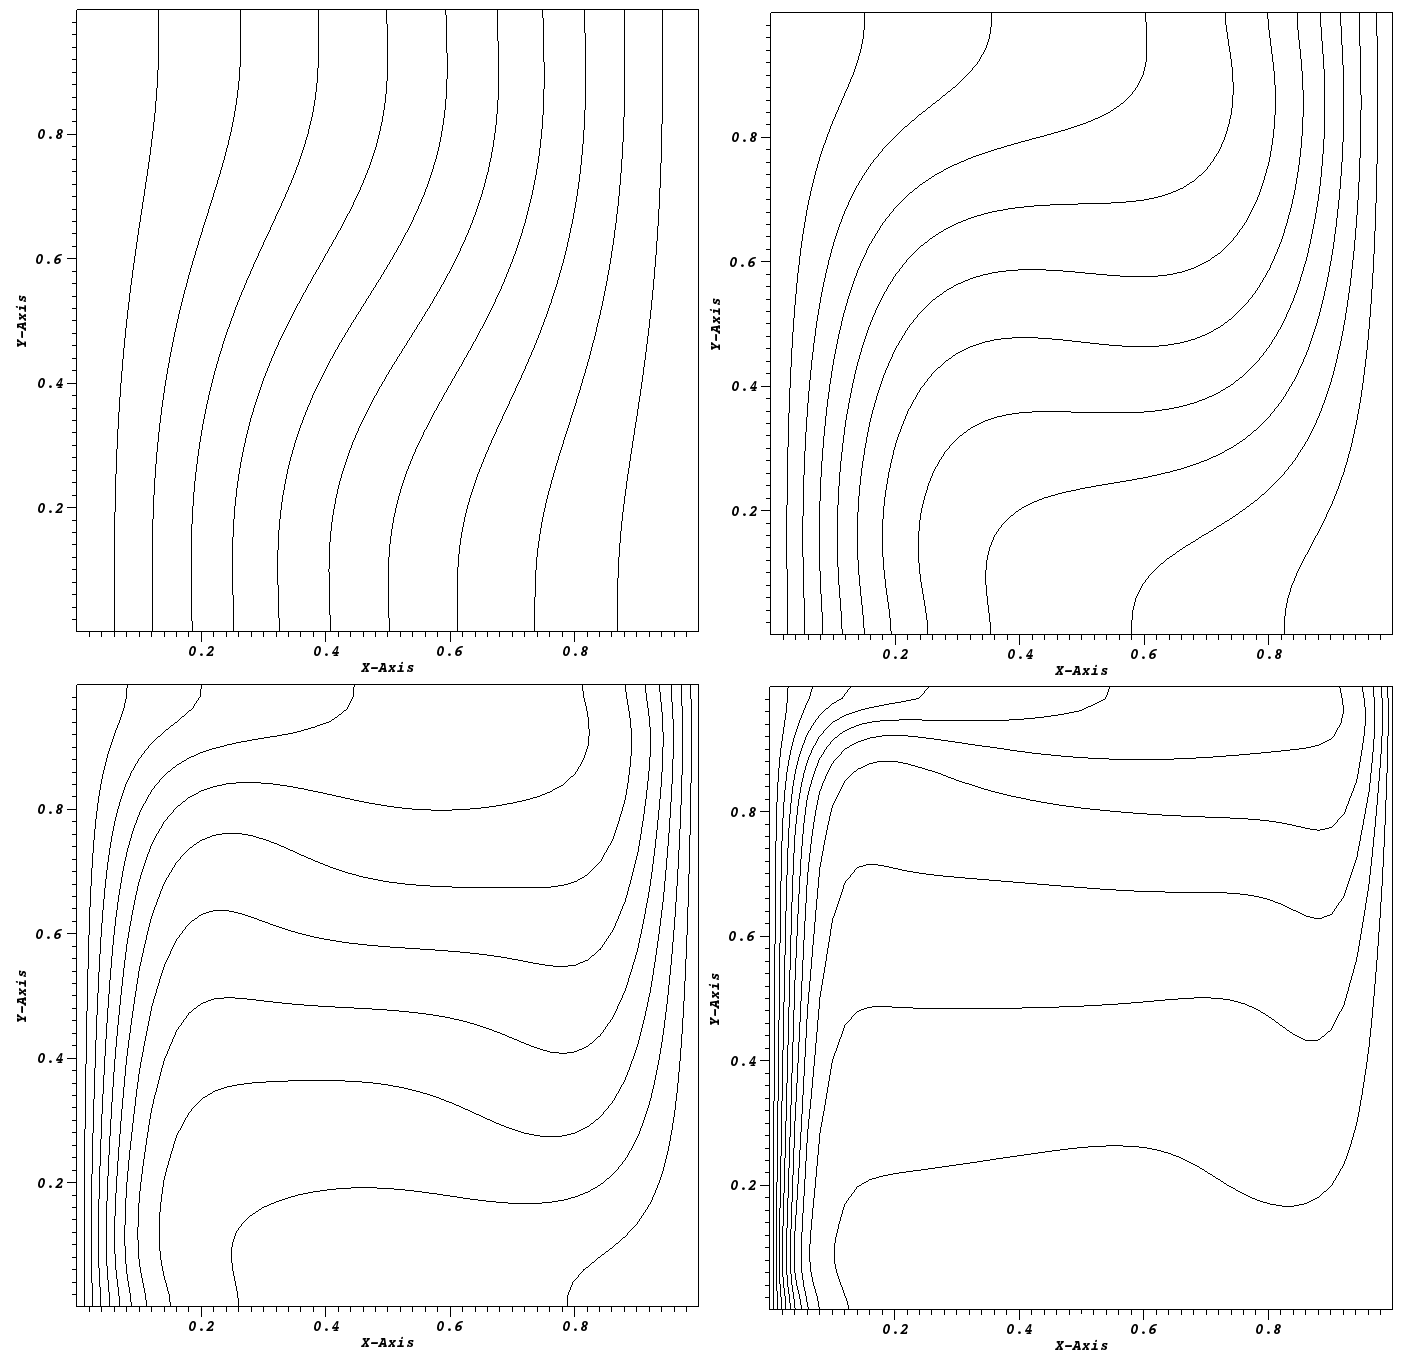
\includegraphics[width=6in]{chapters/nonlinear_problem/convection_isotherms.png}
  \end{center}
  \caption{\textbf{Isotherms from solution to the thermal convection
      cavity problem.} \textit{Top left: Ra = \sn{1}{3}; Top right: Ra
      = \sn{1}{4}; Bottom left: Ra = \sn{1}{5}; Bottom left: Ra =
      \sn{1}{6}. Isotherms on unit temperature scale from 0 to 1 with
      10 uniformly spaced curves for each calculation. These results
      were computed with the Drekar fluid code and FANM.}}
  \label{fig:convection_isotherms}
\end{figure}

\clearpage

\subsection{Lid Driven Cavity Problem}
\label{subsec:lid_driven_cavity}
To study performance for flow driven by inertial forces, the second
benchmark problem given by Ghia \cite{ghia_high-re_1982} incorporates
a driver for the flow to introduce higher Reynolds numbers into the
system, providing more inertial force to overcome the viscous forces
in the fluid. The setup for this problem is equally simple, containing
only the Dirichlet conditions as given in
Figure~\ref{fig:lid_driven_cavity} and is only applied to the mass and
momentum equations on the unit square.

\begin{figure}[t!]
  \begin{center}
    \scalebox{1.5}{
      \input{chapters/nonlinear_problem/lid_driven_cavity.pdftex_t} }
  \end{center}
  \caption{\textbf{Problem setup for the lid driven cavity benchmark.}
    \textit{Dirichlet conditions of zero are set for the velocity on
      the left and right and bottom while the Dirichlet condition set
      on the top provides a driving force on the fluid.}}
  \label{fig:lid_driven_cavity}
\end{figure}

The top boundary condition will provide a driver for the flow and its
variation will in turn vary the Reynolds number of the fluid. An
increased velocity will generate more inertial forces in the fluid,
which will overcome the viscous forces and again increase the
influence of the nonlinear terms in Eq~(\ref{eq:ns_momentum}). Shadid
used Reynolds numbers up to \sn{1}{4} for this benchmark problem.

Isocurves of the velocity magnitudes are given in
Figure~\ref{fig:driven_velocity_isocurves} for solutions to the lid
driven cavity problem at Reynolds numbers of 100, 300, 500 and
700. Increasing the velocity on the top boundary of the problem drives
up the Reynolds number of the system making it more difficult to
solve. More rotation of the fluid is induced by inertial forces and we
begin to see some additional vortexes form besides the primary vortex
near the center of the box.

\begin{figure}[t!]
  \begin{center}
    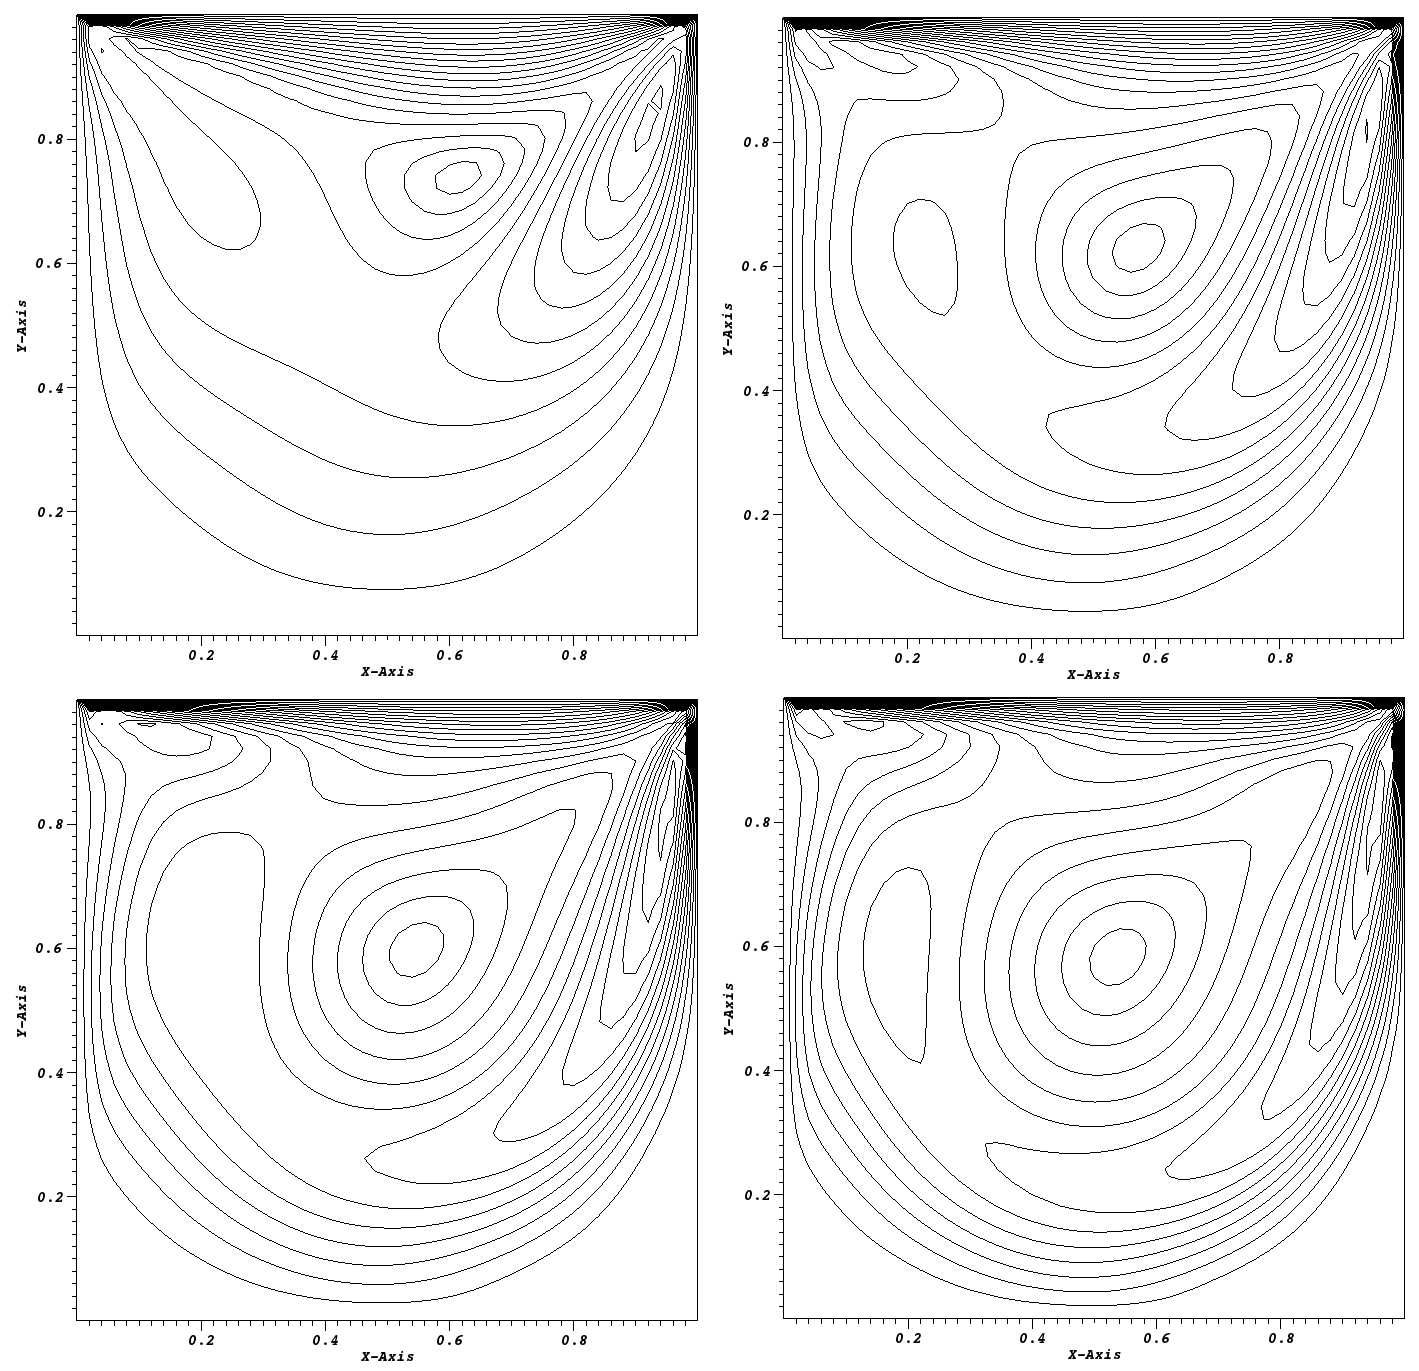
\includegraphics[width=6in]{chapters/nonlinear_problem/driven_velocity_isocurves.png}
  \end{center}
  \caption{\textbf{Velocity magnitude isocurves from solution to the
      lid driven cavity problem.} \textit{Top left: Re = 100; Top
      right: Re= 300; Bottom left: Re = 500; Bottom left: Re =
      700. Isocurves on unit velocity scale from 0 to 1 with 20
      uniformly spaced curves for each calculation. These results were
      computed with the Drekar fluid code and FANM.}}
  \label{fig:driven_velocity_isocurves}
\end{figure}

\clearpage

\subsection{Backward-Facing Step Problem}
\label{subsubsec:backward_facing_step}
The third benchmark was generated by Gartling in 1990 and consists of
both flow over a backward step and an outflow boundary condition
\cite{gartling_test_1990}. Using the mass and momentum equations
while neglecting the energy equation, this problem utilizes a longer
domain with a 1/25 aspect ratio used for this work\footnote{The
  literature on this benchmark suggests using a domain with a 1/30
  aspect ratio to reduce the effect of the outflow boundary condition
  on the upstream recirculation zones. Using a 1/25 aspect ratio for
  this work was not observed to disturb the recirculation zones and
  was therefore used to reduce memory pressure on the FANM solver.}
with the boundary conditions as shown in
Figure~\ref{fig:backward_facing_step}.

\begin{figure}[t!]
  \begin{center}
    \scalebox{1.2}{
      \input{chapters/nonlinear_problem/backward_facing_step.pdftex_t} }
  \end{center}
  \caption{\textbf{Problem setup for the backward facing step
      benchmark.} \textit{Zero velocity boundary conditions are
      applied at the top and bottom of the domain while the outflow
      boundary condition on the right boundary is represented by zero
      stress tensor components in the direction of the flow. For the
      inlet conditions, the left boundary is split such that the top
      half has a fully formed parabolic flow profile and the bottom
      half has a zero velocity condition, simulating flow over a
      step. The $H$ parameter given in the parabolic inlet condition
      is the width of the inlet.}}
  \label{fig:backward_facing_step}
\end{figure}

In this problem, the inflow condition is specified by a fully-formed
parabolic flow profile over a zero velocity boundary representing a
step. For this work, a slightly different parabolic formulation for
the inlet velocities was used than in the benchmark. In the benchmark
solutions, the average velocity in the parabola was 2/3 that of the
maximum velocity while the formula given in
Figure~\ref{fig:backward_facing_step} produces a more plug-like flow
with an average velocity 3/4 that of the maximum velocity. The flow
over this step will generate a recirculating backflow under the inlet
flow towards the step and at higher Reynolds numbers a recirculation
zone will form farther downstream from the step. As in the lid driven
cavity problem, the nonlinear behavior of this benchmark and the
difficulty in obtaining a solution is dictated by the Reynolds number
of the fluid.

Figure~\ref{fig:step_velocity_isocurves} gives the velocity magnitude
contours for solutions to this problem with Reynolds numbers of 200,
300, 400, and 500. As the Reynolds number increases, note the
downstream recirculation zone beginning to form in the upper right
corner of the solution plots where the velocity isocurves are
depressed. In Shadid's work, Reynolds numbers up to 800 were used.

\begin{figure}[t!]
  \begin{center}
    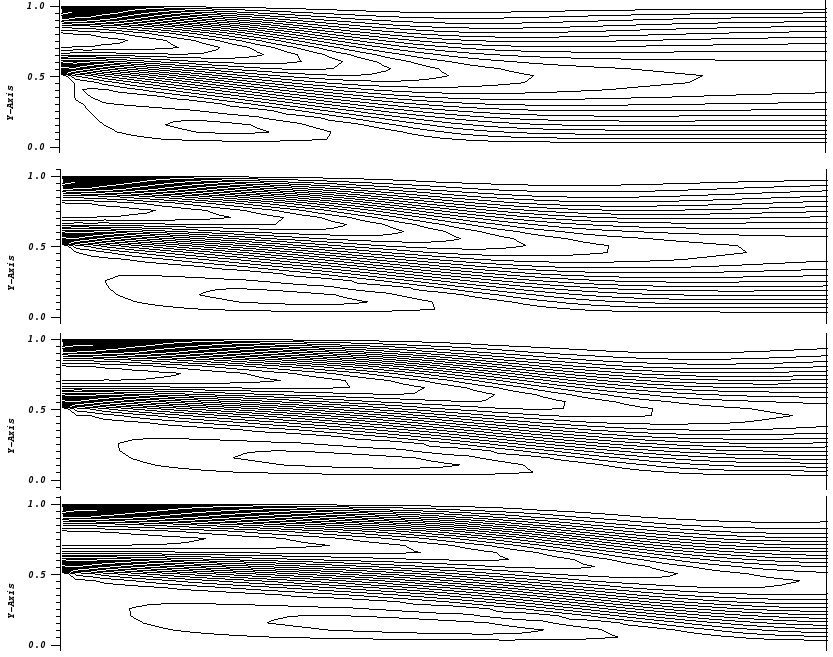
\includegraphics[width=6in]{chapters/nonlinear_problem/step_velocity_isocurves.png}
  \end{center}
  \caption{\textbf{Velocity magnitude isocurves from solution to the
      backward facing step problem.} \textit{From top to bottom: Re =
      200, Re = 300, Re = 400, Re = 500. Isocurves on unit velocity
      scale from 0 to 1 with 20 uniformly spaced curves for each
      calculation. The depression forming in the upper right portion
      of visible flow is the second vortex. These results were
      computed with the Drekar fluid code and FANM.}}
  \label{fig:step_velocity_isocurves}
\end{figure}

\clearpage

%%---------------------------------------------------------------------------%%
\section{FANM Verification\ }
\label{sec:fanm_verification}

For each of the benchmark problems, we will present the results of
computations using FANM and compare them to results using a
Newton-Krylov method in order to verify the correctness of FANM and
its applicability to fluid problems. Given the difficulty of these
benchmark problems, the linear solve at each Newton step was
preconditioned with an algebraic multigrid method\footnote{The ML
  algebraic multigrid library in the Trilinos scientific computing
  libraries \cite{heroux_overview_2005} was used for all problems.}, a
common technique for preconditioning these equations
\cite{ghia_high-re_1982,evans_enhanced_2007}. The preconditioner is
reconstructed at every Newton step for the new Jacobian and used on
the right as outlined in
\S~\ref{subsubsec:general_mcsa_preconditioning}. Without multigrid
preconditioning, the residual in MCSA was observed to
stagnate. Typically this happens because the Richardson iteration and
subsequently the Neumann series will quickly dampen the higher order
error modes on the scale of the computational grid used to solve the
problem but will reduce lower order error modes at a considerably
lower rate. In terms of Monte Carlo, this stagnation manifests itself
in histories that simply do no terminate and therefore no solution is
acquired. For many of the problems presented here, it is likely that a
more physics-based preconditioning strategy such as those presented in
\cite{evans_development_2006,evans_enhanced_2007} will yield better
results for more difficult problems. However, in this work we will
restrict our attention to multigrid for simplicity.

For every benchmark calculation, both FANM and Newton-Krylov were
preconditioned with the same multigrid parameters such that the
conditioning of the system would not be a factor in the verification
of the method or the performance comparison in the following
section. With FANM, this preconditioning was required to reduce the
spectral radius of the Jacobian operators generated at each Newton
step. This preconditioning was also required to obtain good
convergence properties for the Newton-Krylov solutions although it was
not necessary for their convergence. In addition, the same nonlinear
solver parameters including globalization and forcing term strategies
were used for both methods with a \sn{1}{-12} norm for the nonlinear
residual set as the nonlinear convergence criteria. As with the
radiation transport calculations in the previous chapter, algebraic
preconditioning with the multigrid method results in dense linear
systems. To mitigate this, the reduced domain approximation was again
applied to the Monte Carlo solution within the MCSA solve occurring at
each nonlinear iteration. The values used for the approximation will
be given for each benchmark problem.

Results in this and the following section were produced by the Drekar
multiphysics code base being developed at Sandia National Laboratories
for fluid flow and other multiple physics simulations
\cite{pawlowski_drekar_2012}. Drekar is a massively parallel physics
framework that utilizes a finite element formulation of the
Navier-Stokes equations and Newton-Krylov methods with Jacobian
generation through automatic differentiation. To achieve the results
presented here, a Monte Carlo solver generated for this work was
injected into the nonlinear solver sequence within Drekar to form an
implementation of the FANM method. For the Newton-Krylov solutions,
the same implementation of GMRES used for the $SP_N$ verification from
the Trilinos scientific computing library Aztec
\cite{heroux_overview_2005} was also used here as a means of
comparison and FANM benchmarking.

\subsection{Thermal Convection Cavity Results}
\label{subsec:thermal_convection_verification}

A Drekar model of thermal convection cavity problem was solved using
both the Newton-Krylov solver and the FANM solver for Rayleigh numbers
of \sn{1}{3}, \sn{1}{4}, \sn{1}{5} and \sn{1}{6} on a $50 \times 50$
square grid. Table~\ref{tab:thermal_convection_parameters} gives the
physical parameters of the problem and
Table~\ref{tab:convection_mcsa_parameters} gives the MCSA solver
parameters used within the FANM method. Variation in the Rayleigh
number of the system was achieved by keeping the parameters given in
Table~\ref{tab:thermal_convection_parameters} constant and varying the
temperature of the hot side of the cavity. In addition to multigrid
preconditioning for the linear solution at each Newton step,
backtracking as outlined in Shadid's work \cite{shadid_inexact_1997}
was used as a means of globalization to assist the Newton correction
computation while the forcing term at all Rayleigh numbers but
\sn{1}{6} was computed at each Newton step using
Eq~\ref{eq:shadid_forcing}. At a Rayleigh number of \sn{1}{6}, a
constant forcing term of \sn{1}{-4} was use to give better convergence
properties.

\begin{table}[h!]
  \begin{center}
    \begin{tabular}{lcc}\hline\hline
      \multicolumn{1}{l}{Parameter}& 
      \multicolumn{1}{c}{Value}&
      \multicolumn{1}{c}{Units}\\\hline
      $x_{min}$ & 0.0 & $m$ \\
      $x_{max}$ & 1.0 & $m$ \\
      $y_{min}$ & 0.0 & $m$ \\
      $y_{max}$ & 1.0 & $m$ \\
      $N_x$ & 50 & - \\
      $N_y$ & 50 & - \\
      $DOFs$ & 10404 & - \\
      Initial Temperature & 0.0 & $K$ \\
      Density & 1.0 & $kg / m^3$ \\
      Specific Heat & 1.0 & J / $(kg \times K)$ \\
      Dynamic Viscosity & 0.71 & $(N \times s) / m^2$ \\
      Thermal Conductivity & 1.0 & $W / (m \times K)$ \\
      Thermal Expansion Coefficient & 1000 & $1 / K$ \\
      Thermal Diffusivity & 1.0 & $m^2 / s$ \\
      Kinematic Viscosity & 0.71 & $m^2 / s$ \\
      Gravitational Acceleration & 10 & $m / s^2$ \\
      Cavity Characteristic Length & 1.0 & $m$ \\
      Prandtl Number & 0.71 & - \\
      %%
      \hline\hline
    \end{tabular}
  \end{center}
  \caption{\textbf{Thermal convection cavity FANM verification model
      problem parameters.}  \textit{The Navier-Stokes equations in 2
      dimensions are used for the model problem. The Rayleigh number
      is varied by modifying the hot boundary temperature to induce
      larger temperature gradients and buoyancy-driven flow.}}
  \label{tab:thermal_convection_parameters}
\end{table}

\begin{table}[h!]
  \begin{center}
    \begin{tabular}{lc}\hline\hline
      \multicolumn{1}{l}{Parameter}& 
      \multicolumn{1}{c}{Value}\\\hline
      Histories & 500,000 per iteration \\
      Weight Cutoff & \sn{1}{-2} \\
      Fixed Point Iteration & Richardson \\
      Estimator & Adjoint Collision \\
      Reduced Domain Fill Level & 200 \\
      %%
      \hline\hline
    \end{tabular}
  \end{center}
  \caption{\textbf{Thermal convection cavity FANM verification MCSA
      solver parameters.} \textit{No relaxation parameters or variance
      reduction techniques were used with MCSA other than the reduced
      domain approximation.}}
  \label{tab:convection_mcsa_parameters}
\end{table}

At each Rayleigh number the fluid velocity in the x and y directions,
fluid pressure, and fluid temperature values calculated with FANM were
verified by computing the point-wise absolute difference with the
Newton-Krylov results. No variation in the solution was noted for each
of the computations larger than the floating point tolerance reported
by Drekar with an absolute difference value of zero computed at all
spatial locations for each physical quantity.

\subsection{Lid Driven Cavity Results}
\label{subsec:lid_driven_verification}

A Drekar model of thermal convection cavity problem was solved using
both the Newton-Krylov solver and the FANM solver for Reynolds numbers
of 100, 300, 500, and 700 on a $50 \times 50$ square
grid. Table~\ref{tab:lid_driven_parameters} gives the physical
parameters of the problem and Table~\ref{tab:driven_mcsa_parameters}
gives the MCSA solver parameters used within the FANM
method. Variation in the Reynolds number of the system was achieved by
keeping the parameters given in Table~\ref{tab:lid_driven_parameters}
fixed and varying the fluid velocity in the $x$ direction on the top
boundary. In addition to multigrid preconditioning for the linear
solution at each Newton step, a polynomial line search method was used
as a means of globalization, assisting the Newton correction
computation as outlined by Pawlowski in
\cite{pawlowski_globalization_2006} while the forcing term was again
computed using Eq~\ref{eq:shadid_forcing} at all Reynolds numbers.

\begin{table}[h!]
  \begin{center}
    \begin{tabular}{lcc}\hline\hline
      \multicolumn{1}{l}{Parameter}& 
      \multicolumn{1}{c}{Value}&
      \multicolumn{1}{c}{Units}\\\hline
      $x_{min}$ & 0.0 & $m$ \\
      $x_{max}$ & 1.0 & $m$ \\
      $y_{min}$ & 0.0 & $m$ \\
      $y_{max}$ & 1.0 & $m$ \\
      $N_x$ & 50 & - \\
      $N_y$ & 50 & - \\
      $DOFs$ & 7803 & - \\
      Density & 1.0 & $kg / m^3$ \\
      Dynamic Viscosity & 0.71 & $(N \times s) / m^2$ \\
      Kinematic Viscosity & 0.71 & $m^2 / s$ \\
      Cavity Characteristic Length & 1.0 & $m$ \\
      %%
      \hline\hline
    \end{tabular}
  \end{center}
  \caption{\textbf{Lid driven cavity FANM verification model
      problem parameters.}  \textit{The Navier-Stokes equations in 2
      dimensions are used for the model problem. The Reynolds number
      is varied by modifying the velocity magnitude on the upper
      boundary to induce flow driven by inertial forces.}}
  \label{tab:lid_driven_parameters}
\end{table}

\begin{table}[h!]
  \begin{center}
    \begin{tabular}{lc}\hline\hline
      \multicolumn{1}{l}{Parameter}& 
      \multicolumn{1}{c}{Value}\\\hline
      Weight Cutoff & \sn{1}{-2} \\
      Fixed Point Iteration & Richardson \\
      Estimator & Adjoint Collision \\
      Histories, Re=100 & 500,000 per iteration \\
      Histories, Re=300 & 500,000 per iteration \\
      Histories, Re=500 & 500,000 per iteration \\
      Histories, Re=700 & 1,000,000 per iteration \\
      Reduced Domain Fill Level, Re=100 & 200 \\
      Reduced Domain Fill Level, Re=300 & 200 \\
      Reduced Domain Fill Level, Re=500 & 200 \\
      Reduced Domain Fill Level, Re=700 & 300 \\
      %%
      \hline\hline
    \end{tabular}
  \end{center}
  \caption{\textbf{Lid driven cavity FANM verification MCSA solver
      parameters.} \textit{No relaxation parameters or variance
      reduction techniques were used with MCSA other than the reduced
      domain approximation. Different values of fill level for the
      reduced domain approximation and histories per iteration were
      used at different Reynolds numbers due to convergence
      requirements.}}
  \label{tab:driven_mcsa_parameters}
\end{table}

In the literature on this benchmark, solutions at Reynolds numbers of
up to \sn{1}{4} were achieved using a variety of nonlinear solution
techniques. With the FANM method, at Reynolds numbers above 700
convergence of the linear iterations could not be achieved regardless
of how aggressive the multigrid preconditioner was set. In these cases,
the Jacobian operators are ill-conditioned enough that even GMRES
converges slowly relative to the thermal convection cavity
benchmark. Therefore, the spectral radius limitation on MCSA is
extremely prohibitive in this case and others where transport driven
by inertial forces is dominant. Because of this, only solutions to
the lid driven cavity benchmark at Reynolds numbers of up to 700 are
presented.

At each Reynolds number the fluid velocity in the x and y directions
and fluid pressure values calculated with FANM were verified by
computing the point-wise absolute difference with the Newton-Krylov
results. No variation in the solution was noted for each of the
computations larger than the floating point tolerance reported by
Drekar with an absolute difference value of zero computed at all
spatial locations for each physical quantity.

\subsection{Backward Facing Step Results}
\label{subsec:backward_step_verification}

A Drekar model of the backward facing step problem was solved using
both the Newton-Krylov solver and the FANM solver for Reynolds numbers
of 200, 300, 400, and 500 on a $20 \times 250$ rectangular
grid. Table~\ref{tab:backward_step_parameters} gives the physical
parameters of the problem and Table~\ref{tab:step_mcsa_parameters}
gives the MCSA solver parameters used within the FANM
method. Variation in the Reynolds number of the system was achieved by
keeping the parameters given in
Table~\ref{tab:backward_step_parameters} fixed and varying the maximum
fluid velocity in the parabolic inlet condition. In addition to
multigrid preconditioning for the linear solution at each Newton step,
a polynomial line search method was used as a means of globalization
while the forcing term was again computed using Eq~\ref{eq:shadid_forcing}.

\begin{table}[h!]
  \begin{center}
    \begin{tabular}{lcc}\hline\hline
      \multicolumn{1}{l}{Parameter}& 
      \multicolumn{1}{c}{Value}&
      \multicolumn{1}{c}{Units}\\\hline
      $x_{min}$ & 0.0 & $m$ \\
      $x_{max}$ & 25.0 & $m$ \\
      $y_{min}$ & 0.0 & $m$ \\
      $y_{max}$ & 1.0 & $m$ \\
      $N_x$ & 20 & - \\
      $N_y$ & 250 & - \\
      $DOFs$ & 15813 & - \\
      Density & 1.0 & $kg / m^3$ \\
      Dynamic Viscosity & 1.0 & $(N \times s) / m^2$ \\
      Kinematic Viscosity & 1.0 & $m^2 / s$ \\
      Channel Width & 1.0 & $m$ \\
      Step Height & 0.5 & $m$ \\
      %%
      \hline\hline
    \end{tabular}
  \end{center}
  \caption{\textbf{Backward facing step FANM verification model
      problem parameters.}  \textit{The Navier-Stokes equations in 2
      dimensions are used for the model problem. The Reynolds number
      is varied by modifying the maximum velocity magnitude in the
      parabolic inlet condition.}}
  \label{tab:backward_step_parameters}
\end{table}

\begin{table}[h!]
  \begin{center}
    \begin{tabular}{lc}\hline\hline
      \multicolumn{1}{l}{Parameter}& 
      \multicolumn{1}{c}{Value}\\\hline
      Weight Cutoff & \sn{1}{-2} \\
      Fixed Point Iteration & Richardson \\
      Estimator & Adjoint Collision \\
      Histories, Re=200 & 500,000 per iteration \\
      Histories, Re=300 & 500,000 per iteration \\
      Histories, Re=400 & 500,000 per iteration \\
      Histories, Re=500 & 1,000,000 per iteration \\
      Reduced Domain Fill Level, All Re & 200 \\
      %%
      \hline\hline
    \end{tabular}
  \end{center}
  \caption{\textbf{Backward facing step FANM verification MCSA solver
      parameters.} \textit{No relaxation parameters or variance
      reduction techniques were used with MCSA other than the reduced
      domain approximation. The same fill level for the reduced domain
      approximation was used at every Reynolds numbers and different
      histories per iteration were used at different Reynolds numbers
      due to convergence requirements.}}
  \label{tab:step_mcsa_parameters}
\end{table}

In the literature on this benchmark, solutions at Reynolds numbers of
up to 800 were achieved using a variety of nonlinear solution
techniques. In identical fashion to the lid driven cavity problem, at
Reynolds numbers above 500 convergence of the linear iterations could
not be achieved with FANM regardless of how aggressive the multigrid
preconditioner was set. In these cases, the Jacobian operators are
again ill-conditioned enough that a spectral radius of less than one
could not be achieved with multigrid preconditioning and several cycle
applications. Therefore, the spectral radius limitation on MCSA is
extremely prohibitive in this case as well and even more so than the
lid driven cavity problem where solutions at higher Reynolds numbers
were achieved. Because of this, only solutions to the backward facing
step benchmark at Reynolds numbers of up to 500 are presented.

At each Reynolds number the fluid velocity in the x and y directions
and fluid pressure values calculated with FANM were verified by
computing the point-wise absolute difference with the Newton-Krylov
results. No variation in the solution was noted for each of the
computations larger than the floating point tolerance reported by
Drekar with an absolute difference value of zero computed at all
spatial locations for each physical quantity.

%%---------------------------------------------------------------------------%%
\section{FANM Performance Comparison to Conventional Methods\ }
\label{sec:fanm_comparison}

Using the benchmarks from the verification, we now compare the
performance of the FANM method against a conventional Newton-Krylov
(NK) method. For each benchmark, we will analyze the iterative
performance of both the Newton solver and the linear solver used to
compute the Newton correction vector at each step. Limiting the number
of nonlinear iterations required for solution is critical for
efficiency as nonlinear function evaluations, Jacobian generation, and
preconditioner construction are typically required at every Newton
iteration. In addition, timing results will also be discussed. To
quantify the acceleration provided by the residual Monte Carlo
component of MCSA, each calculation was also performed using the same
Newton method but with a preconditioned Richardson iteration as the
linear solution technique to give a Newton-Richardson (NR) scheme. For
all cases the Richardson iteration was preconditioned with multigrid
in the same way as GMRES and MCSA.

\subsection{Thermal Convection Cavity Results}
\label{subsec:thermal_convection_comparison}

At each Rayleigh number used for the thermal convection cavity
problem, Table~\ref{tab:convection_nonlinear_iter_comparison} gives
the number of Newton iterations required for convergence for each
method.  For all Rayleigh numbers except \sn{1}{5} the number of
Newton iterations required to converge is the same while the \sn{1}{5}
result required an extra FANM iteration. This is due to the fact that
the convergence of the linear residual has a strong effect on the
convergence of the nonlinear residual. For nonlinear calculations,
this is much stronger than the effect on the convergence of the
eigenvalue in the $SP_N$ computations where we always observed that
identical numbers of k-eigenvalue iterations were required to converge
each variation of the problem.

As outlined in our discussion on inexact Newton methods, depending on
how converged the linear residual is at each step, it is possible to
throw off the nonlinear iteration and decrease iterative
performance. Although the same preconditioner was used with both the
Newton-Krylov and FANM calculations, the convergence properties of
MCSA and GMRES are different and we therefore expect them to produce
different results at each nonlinear iteration which will in turn
affect the forcing term calculation. If they are different enough, it
is possible that another Newton iteration may be required. Even
considering the extra Newton iteration, the solutions are converged to
effectively the same residual norm tolerance and produce the same
results as provided by the verification.

Figure~\ref{fig:ra1e5_convergence} gives the nonlinear residual
behavior for the \sn{1}{5} Rayleigh number case that required the
extra FANM iteration. We see that the extra iteration comes from
slightly slower quadratic convergence with FANM for this particular
case. The difference in convergence of the nonlinear problem comes
from the fact that the same multigrid preconditioner parameters are
used for this case as for the \sn{1}{3} and \sn{1}{4} Rayleigh number
cases for the linear solutions. Using the same preconditioner for the
harder \sn{1}{5} case means that the problem is still growing in
difficulty even though it is preconditioned in an identical
manner. This means that GMRES at each Newton step is converging the
linear residual to a smaller tolerance than MCSA as the forcing terms
adapt to the convergence of the method over the course of nonlinear
iterations. For this problem, tighter convergence of the linear model
at later Newton steps also improved convergence of nonlinear model,
resulting in the extra FANM iteration.

As the Rayleigh number increases, the problem becomes more difficult
to solve and therefore a more aggressive preconditioner should
maintain iterative performance of the nonlinear method. This was
observed to be true for the \sn{1}{6} Rayleigh number case. For this
calculation, the number of multigrid cycle applications was increased
to 3 from 1 and FANM converged in the same number of nonlinear
iterations as the Newton-Krylov method.

\begin{table}[h!]
  \begin{center}
    \begin{tabular}{cccc}\hline\hline
      \multicolumn{1}{c}{Rayleigh Number}& 
      \multicolumn{1}{c}{NK Iterations}&
      \multicolumn{1}{c}{FANM Iterations}&
      \multicolumn{1}{c}{NR Iterations}\\
      \hline
      \sn{1}{3} & 5 & 5 & 5\\
      \sn{1}{4} & 7 & 7 & 7\\
      \sn{1}{5} & 9 & 10 & 9\\
      \sn{1}{6} & 11 & 11 & 11\\
      %%
      \hline\hline
    \end{tabular}
  \end{center}
  \caption{\textbf{Thermal convection cavity nonlinear iteration
      results for the performance comparison.} \textit{The results
      presented here were obtained from the benchmark verification
      calculations.}}
  \label{tab:convection_nonlinear_iter_comparison}
\end{table}

\begin{figure}[t!]
  \begin{center}
    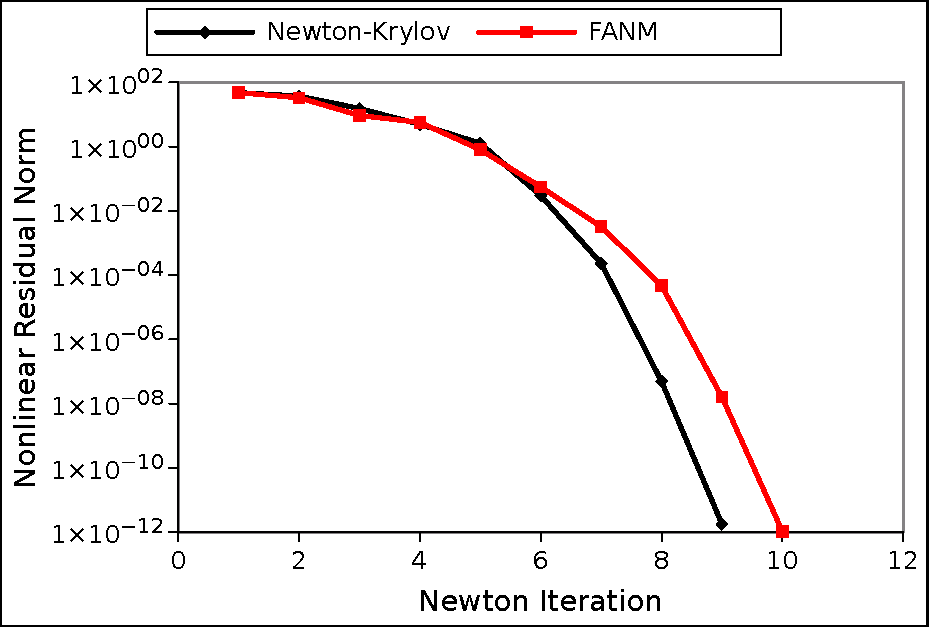
\includegraphics[width=6in]{chapters/nonlinear_problem/ra_1e5_convergence.pdf}
  \end{center}
  \caption{\textbf{Thermal convection cavity nonlinear residual norm
      as a function of Newton iteration for the \sn{1}{5} Rayleigh
      number case.} \textit{The FANM calculation required an
      additional nonlinear iteration to converge.}}
  \label{fig:ra1e5_convergence}
\end{figure}

In addition to nonlinear iterative performance, performance of the
inner linear solves is also of interest. Here, we seek to minimize the
number of total linear solver iterations over the course of all
nonlinear iterations in order to limit matrix-vector multiplies and
other costly
operations. Table~\ref{tab:convection_linear_iter_comparison} gives
the total number of GMRES, MCSA, and Richardson iterations required to
converge the Newton method at each Rayleigh number used. For all
cases, fewer MCSA iterations were required than GMRES iterations to
converge the problem even with both solvers preconditioned with the
same multigrid package and the same parameters. For the \sn{1}{6}
Rayleigh number case where a constant forcing term of \sn{1}{-4} was
kept, this difference is most drastic with FANM requiring only 64\% of
the linear iterations required by the Newton-Krylov scheme with the
linear solver iterations at every nonlinear iteration given for this
case in Figure~\ref{fig:ra1e6_linear_iters}. Even the \sn{1}{5}
Rayleigh number case that required more Newton iterations required 5
fewer MCSA iterations to converge than GMRES iterations. In all cases,
MCSA improved on the iterative performance of using only the
Richardson iteration through the residual Monte Carlo acceleration. If
the performance of the MCSA implementation used here were to be
potentially optimized in the future, this improved iterative
performance could also mean improved time to solution.

\begin{table}[h!]
  \begin{center}
    \begin{tabular}{cccc}\hline\hline
      \multicolumn{1}{c}{Rayleigh Number}&
      \multicolumn{1}{c}{GMRES Iterations}&
      \multicolumn{1}{c}{MCSA Iterations}&
      \multicolumn{1}{c}{Richardson Iterations}\\
      \hline
      \sn{1}{3} & 23 & 18 & 38 \\
      \sn{1}{4} & 23 & 17 & 34 \\
      \sn{1}{5} & 25 & 20 & 34 \\
      \sn{1}{6} & 39 & 25 & 48  \\
      %%
      \hline\hline
    \end{tabular}
  \end{center}
  \caption{\textbf{Thermal convection cavity total sum of linear
      iterations for all nonlinear iterations.} \textit{The results
      presented here were obtained from the benchmark verification
      calculations.}}
  \label{tab:convection_linear_iter_comparison}
\end{table}

\begin{figure}[t!]
  \begin{center}
    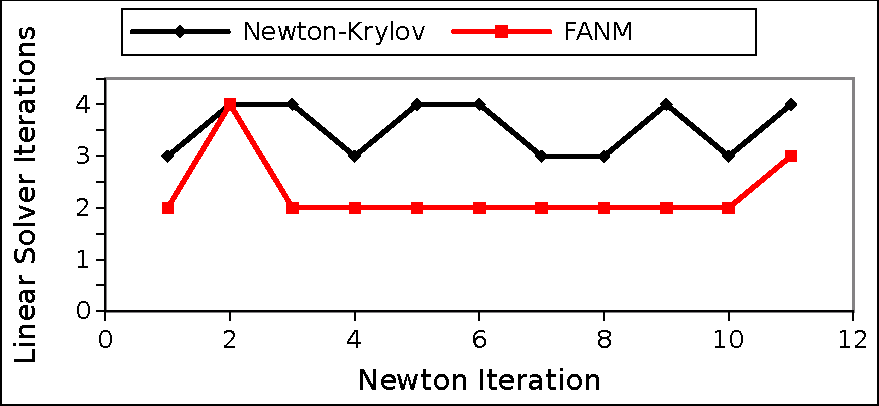
\includegraphics[width=6in]{chapters/nonlinear_problem/convection_ra1e6_iters.pdf}
  \end{center}
  \caption{\textbf{Thermal convection cavity linear solver iterations
      as a function of Newton iteration for the \sn{1}{6} Rayleigh
      number case.} \textit{MCSA shows better iterative performance
      than GMRES at all but the second nonlinear iteration and MCSA
      always accelerated the Richardson iteration. The forcing term
      was fixed at \sn{1}{-4} at all nonlinear iterations.}}
  \label{fig:ra1e6_linear_iters}
\end{figure}

Although the iterative performance of FANM is excellent for the
thermal convection cavity problem, the explicit preconditioning
strategy causes the same issues as was observed for the $SP_N$
equations in the previous
chapter. Table~\ref{tab:convection_speedup_comparison} gives the
speedup of the Newton-Krylov method over FANM. For all Rayleigh
numbers, we see a fairly constant speedup of O(400) when using
Newton-Krylov over FANM meaning that the implementation of the FANM
method used here is significantly slower. 

\begin{table}[h!]
  \begin{center}
    \begin{tabular}{cc}\hline\hline
      \multicolumn{1}{c}{Rayleigh Number}& 
      \multicolumn{1}{c}{Newton-Krylov Speedup}\\
      \hline
      \sn{1}{3} & 338 \\
      \sn{1}{4} & 336 \\
      \sn{1}{5} & 346 \\
      \sn{1}{6} & 465 \\
      %%
      \hline\hline
    \end{tabular}
  \end{center}
  \caption{\textbf{Thermal convection cavity Newton-Krylov speedup
      over FANM method.} \textit{Speedup values are rounded to the
      nearest integer. The results presented here were obtained from
      the benchmark verification calculations.}}
  \label{tab:convection_speedup_comparison}
\end{table}

As the inexact Newton scheme in Drekar was modified by simply swapping
out the linear solver used at each Newton step, this increased compute
time is coming directly from using MCSA as the linear solver and the
overhead due to preconditioning. When preconditioning overhead for the
$SP_N$ equations was considered as shown by the data in
Figure~\ref{fig:spn_comparison_prec_time}, a similar speedup of
approximately two orders of magnitude was noted between the Krylov
methods and MCSA showing consistency between those results and the
convection cavity benchmark results presented. In addition, the fairly
constant speedup values as a function of the primary problem parameter
show that FANM has effectively the same time complexity as a
Newton-Krylov method and the implementation timings simply differ by a
constant value, also consistent with the $SP_N$ observations.

\subsection{Lid Driven Cavity Results}
\label{subsec:lid_driven_comparison}

For the lid driven cavity benchmark, performance results were again
compared between the FANM and Newton-Krylov calculations. In this
case, the nonlinear iterative performance results as given by
Table~\ref{tab:driven_nonlinear_iter_comparison} show that the same
number of Newton iterations were required to converge the 100, 300,
and 500 Reynolds number cases while the FANM calculation with a
Reynolds number of 700 actually converged in 4 fewer iterations. The
nonlinear residual norm as a function of Newton iteration for this
case is given in Figure~\ref{fig:re700_convergence}.

This result can be explained by the fact that as given by
Table~\ref{tab:driven_mcsa_parameters}, although the preconditioner
parameters were the same for both calculations, the MCSA iteration was
pushed harder at a Reynolds number of 700 by doubling the number of
histories used for the computation at each nonlinear iteration. These
extra histories provided better convergence of the linear model at
each iteration and did not result in over-solving, thereby increasing
the convergence rate of the nonlinear model as well. This result is
significant in that it shows increasing the number of histories used
for each MCSA iteration can improve the performance of both linear and
nonlinear convergence. However, further research is required to study
the relationship between the acceleration parameters and the nonlinear
convergence to confirm this for a broader range of problems.

\begin{table}[h!]
  \begin{center}
    \begin{tabular}{cccc}\hline\hline
      \multicolumn{1}{c}{Reynolds Number}& 
      \multicolumn{1}{c}{NK Iterations}&
      \multicolumn{1}{c}{FANM Iterations}&
      \multicolumn{1}{c}{NR Iterations}\\
      \hline
      100 & 6 & 6 & 7\\
      300 & 9 & 9 & 9\\
      500 & 11 & 11 & 11\\
      700 & 14 & 10 & 12\\
      %%
      \hline\hline
    \end{tabular}
  \end{center}
  \caption{\textbf{Lid driven cavity nonlinear iteration
      results for the performance comparison.} \textit{The results
      presented here were obtained from the benchmark verification
      calculations.}}
  \label{tab:driven_nonlinear_iter_comparison}
\end{table}

\begin{figure}[t!]
  \begin{center}
    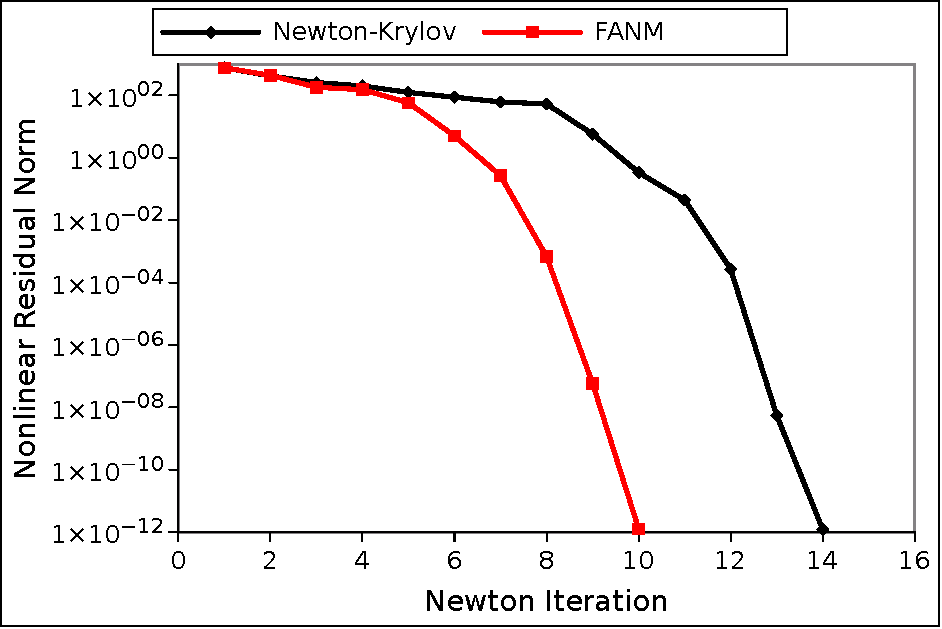
\includegraphics[width=6in]{chapters/nonlinear_problem/re700_convergence.pdf}
  \end{center}
  \caption{\textbf{Lid driven cavity nonlinear residual norm as a
      function of Newton iteration for the 700 Reynolds number case.}
    \textit{The FANM calculation converged in 4 fewer iterations than
      the Newton-Krylov calculation.}}
  \label{fig:re700_convergence}
\end{figure}

The difficulty of this benchmark problem as compared to the thermal
convection cavity problem is readily apparent in the linear iteration
counts as given by Table~\ref{tab:driven_linear_iter_comparison}. Lid
driven cavity results show that the linear models were significantly
more ill-conditioned, requiring many more MCSA and GMRES
iterations. For all cases except the 700 Reynolds number case, many
more MCSA iterations were required to converge with the observed GMRES
iteration count 64\% of that observed for MCSA when looking at the 100
Reynolds number case. For the 700 Reynolds number case, fewer MCSA
iterations were observed due to the fact that 4 fewer nonlinear
iterations were performed. The average number of linear iterations per
nonlinear iteration was still much larger for the FANM
calculations. In all cases, MCSA improved on the iterative performance
of using only the Richardson iteration through the residual Monte
Carlo acceleration even considering the cases with Reynolds numbers of
100 and 700 where an extra Newton-Richardson iteration was required to
converge the nonlinear model.

\begin{figure}[t!]
  \begin{center}
    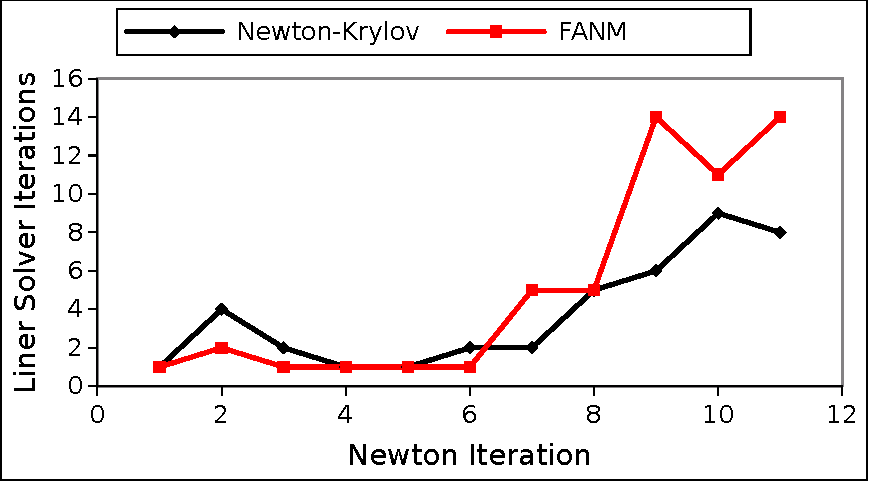
\includegraphics[width=6in]{chapters/nonlinear_problem/driven_re500_iters.pdf}
  \end{center}
  \caption{\textbf{Lid driven cavity linear solver iterations as a
      function of Newton iteration for the 500 Reynolds number case.}
    \textit{More MCSA iterations were required to converge the linear
      models at later Newton iterations due to smaller forcing
      terms.}}
  \label{fig:driven_re500_iters}
\end{figure}

\begin{figure}[t!]
  \begin{center}
    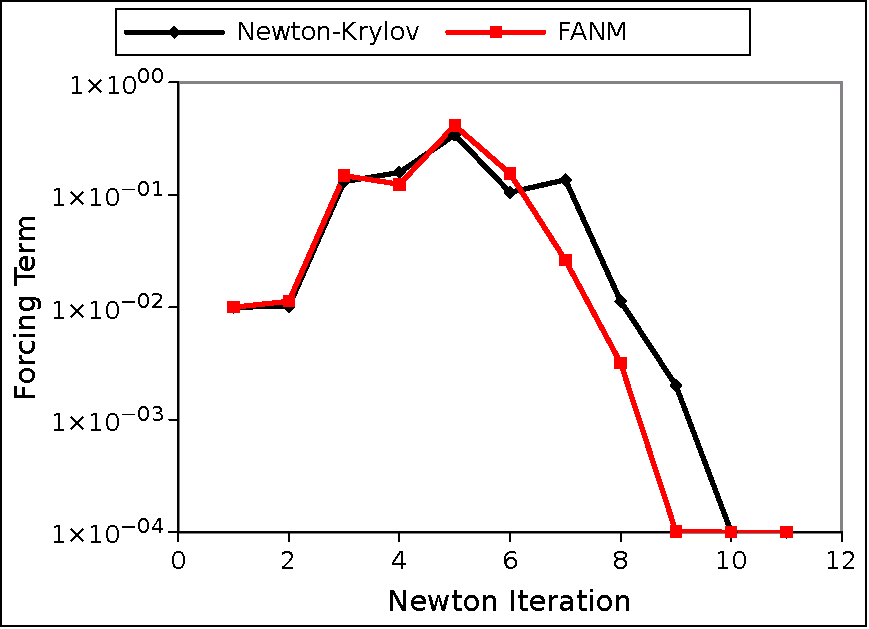
\includegraphics[width=6in]{chapters/nonlinear_problem/driven_re500_forcing.pdf}
  \end{center}
  \caption{\textbf{Lid driven cavity forcing terms as a function of
      Newton iteration for the 500 Reynolds number case.} \textit{Once
      the region of fast quadratic convergence is reached, MCSA
      forcing terms were much smaller.}}
  \label{fig:driven_re500_forcing}
\end{figure}

\begin{table}[h!]
  \begin{center}
    \begin{tabular}{cccc}\hline\hline
      \multicolumn{1}{c}{Reynolds Number}& 
      \multicolumn{1}{c}{GMRES Iterations}&
      \multicolumn{1}{c}{MCSA Iterations}&
      \multicolumn{1}{c}{Richardson Iterations}\\
      \hline
      100 & 27 & 42 & 151\\
      300 & 35 & 52 & 133\\
      500 & 41 & 56 & 154\\
      700 & 21 & 14 & 32\\
      %%
      \hline\hline
    \end{tabular}
  \end{center}
  \caption{\textbf{Lid driven cavity total sum of linear iterations
      for all nonlinear iterations.} \textit{The results presented
      here were obtained from the benchmark verification
      calculations. MCSA always accelerated the Richardson
      iteration.}}
  \label{tab:driven_linear_iter_comparison}
\end{table}

As an additional means of analysis for the linear solver iteration
results, we will look at a case where MCSA performed poorly compared
to GMRES. Consider the linear iterations as a function of nonlinear
iteration given in Figure~\ref{fig:driven_re500_iters} and the forcing
term as a function of nonlinear iteration given in
Figure~\ref{fig:driven_re500_forcing} for the 500 Reynolds number
case. At the later Newton iterations where the region of fast
quadratic convergence is reached, we see that MCSA required many more
iterations to converge than GMRES, accounting for the majority of the
extra iterations. However, we see in the forcing term data that
forcing terms at later Newton iterations for MCSA were much smaller
than those for GMRES. Per Eq~(\ref{eq:newton_stopping_criteria}), this
means that MCSA was converged to a smaller tolerance at these
nonlinear iterations than GMRES and therefore required extra linear
iterations to meet the convergence criteria.

As a final comparison, the timing of both methods was again compared
with the speedup of using the Newton-Krylov solver over FANM reported
in Table~\ref{tab:driven_speedup_comparison}. The speedup values
reported here are of the same magnitude as those reported for the
thermal convection cavity problem and again in agreement with those
observed for the $SP_N$ calculations. Lack of significant variation in
these timing results also point to a qualitatively similar time
complexity for the FANM method as a function of primary problem
parameter relative to the Newton-Krylov method. In all cases, the
preconditioning strategy must be significantly improved along with
implementation optimization to avoid these large overheads.

\begin{table}[h!]
  \begin{center}
    \begin{tabular}{cc}\hline\hline
      \multicolumn{1}{c}{Reynolds Number}& 
      \multicolumn{1}{c}{Newton-Krylov Speedup}\\
      \hline
      100 & 299 \\
      300 & 322 \\
      500 & 288 \\
      700 & 488 \\
      %%
      \hline\hline
    \end{tabular}
  \end{center}
  \caption{\textbf{Lid driven cavity Newton-Krylov speedup over FANM
      method.} \textit{Speedup values are rounded to the nearest
      integer. The results presented here were obtained from the
      benchmark verification calculations.}}
  \label{tab:driven_speedup_comparison}
\end{table}

\clearpage

\subsection{Backward Facing Step Results}
\label{subsec:backward_step_comparison}

The backward step problem exhibited different performance
characteristics than the other two benchmark problems, likely due to
the different geometry and boundary
conditions. Table~\ref{tab:step_nonlinear_iter_comparison} gives the
nonlinear iteration results for this benchmark. At low Reynolds
numbers, FANM converges in fewer nonlinear iterations than the
Newton-Krylov solver. However, as the problem becomes more difficult
to solver at higher rates of flow, the Newton-Krylov solver eventually
converges in fewer nonlinear iterations. We see the same behavior as
well in the linear solver iteration data given by
Table~\ref{tab:step_linear_iter_comparison}. At the 3 lowest Reynolds
numbers, FANM required significantly fewer linear solver iterations to
converge the problem while the ill-conditioned case at a Reynolds
number of 500 is observed to use many more MCSA iterations. For
Reynolds numbers of 200, 300, and 500, FANM also reduced the number of
Newton steps needed when compared to the Newton-Richardson scheme.

\begin{table}[h!]
  \begin{center}
    \begin{tabular}{cccc}\hline\hline
      \multicolumn{1}{c}{Reynolds Number}& 
      \multicolumn{1}{c}{NK Iterations}&
      \multicolumn{1}{c}{FANM Iterations}&
      \multicolumn{1}{c}{NR Iterations}\\
      \hline
      200 & 10 & 9 & 10\\
      300 & 15 & 14 & 15\\
      400 & 10 & 10 & 10\\
      500 & 19 & 20 & 21\\
      %%
      \hline\hline
    \end{tabular}
  \end{center}
  \caption{\textbf{Backward facing step nonlinear iteration
      results for the performance comparison.} \textit{The results
      presented here were obtained from the benchmark verification
      calculations.}}
  \label{tab:step_nonlinear_iter_comparison}
\end{table}

\begin{table}[h!]
  \begin{center}
    \begin{tabular}{cccc}\hline\hline
      \multicolumn{1}{c}{Reynolds Number}& 
      \multicolumn{1}{c}{GMRES Iterations}&
      \multicolumn{1}{c}{MCSA Iterations}&
      \multicolumn{1}{c}{Richardson Iterations}\\
      \hline
      200 & 24 & 13 & 21\\
      300 & 23 & 17 & 21\\
      400 & 18 & 12 & 14\\
      500 & 30 & 52 & 98\\
      %%
      \hline\hline
    \end{tabular}
  \end{center}
  \caption{\textbf{Backward facing step total sum of linear iterations
      for all nonlinear iterations.} \textit{The results presented
      here were obtained from the benchmark verification
      calculations.MCSA always accelerated the Richardson iteration.}}
  \label{tab:step_linear_iter_comparison}
\end{table}

Unlike the lid driven cavity benchmark, the extra linear solver
iterations are not due to the smaller forcing terms but are rather
truly a function of the ill-conditioning of the Jacobian matrices
produced at each Newton step. We see this by comparing the results at
Reynolds numbers of 400 where FANM outperformed Newton-Krylov and 500
where Newton-Krylov outperformed FANM. Linear iterations as a function
of nonlinear iteration given in Figure~\ref{fig:step_re400_iters} and
the forcing term as a function of nonlinear iteration given in
Figure~\ref{fig:step_re400_forcing} for the 400 Reynolds number case
and the same data is given in Figure~\ref{fig:step_re500_iters} and
Figure~\ref{fig:step_re500_forcing} for the 500 Reynolds number
case. For both cases, FANM always has larger forcing terms and should
therefore use fewer MCSA iterations at each Newton step to converge
the linear model if the iterative performance is comparable. This is
indeed the case for the 400 Reynolds number case where FANM used fewer
total linear solver iterations to converge the nonlinear
residual. However, at a Reynolds number of 500 FANM has larger forcing
terms but requires many more MCSA iterations to converge the last 2
Newton steps. Therefore, these extra iterations in this case must come
from ill-conditioning.

We additionally see the effects of ill-conditioned Jacobians when
looking at the acceleration provided by MCSA over using a
preconditioned Richardson iteration. For the first 3 cases, the
acceleration was not as significant as for the other benchmark
problems. In this case, this means that the Richardson iteration and
its acceleration by a stochastic realization of a Richardson iteration
are not doing the bulk of the work in this problem. Rather, the
algebraic multigrid preconditioning is performing more work at each
iteration and therefore the acceleration is smaller. When the system
becomes even more ill-conditioned in the 500 Reynolds number case
the acceleration has more of an impact.

\begin{figure}[t!]
  \begin{center}
    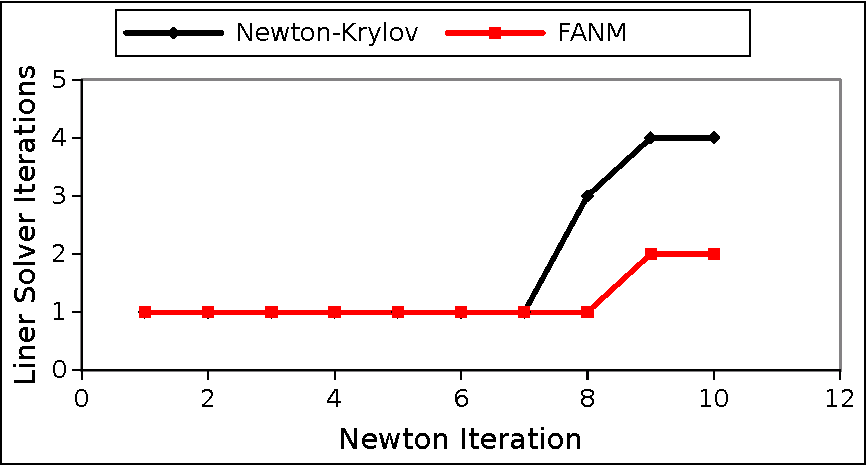
\includegraphics[width=6in]{chapters/nonlinear_problem/step_re400_iters.pdf}
  \end{center}
  \caption{\textbf{Backward facing step linear solver iterations as a
      function of Newton iteration for the 400 Reynolds number case.}
    \textit{More MCSA iterations were required to converge the linear
      models at later Newton iterations due to ill-conditioning of the
      Jacobian matrices.}}
  \label{fig:step_re400_iters}
\end{figure}

\begin{figure}[t!]
  \begin{center}
    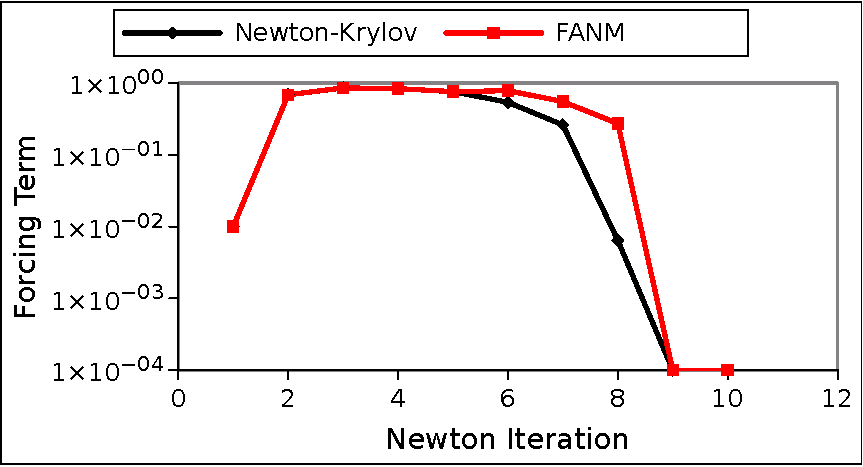
\includegraphics[width=6in]{chapters/nonlinear_problem/step_re400_forcing.pdf}
  \end{center}
  \caption{\textbf{Backward facing step forcing terms as a function of
      Newton iteration for the 400 Reynolds number case.} \textit{FANM
      forcing terms were always larger.}}
  \label{fig:step_re400_forcing}
\end{figure}

\begin{figure}[t!]
  \begin{center}
    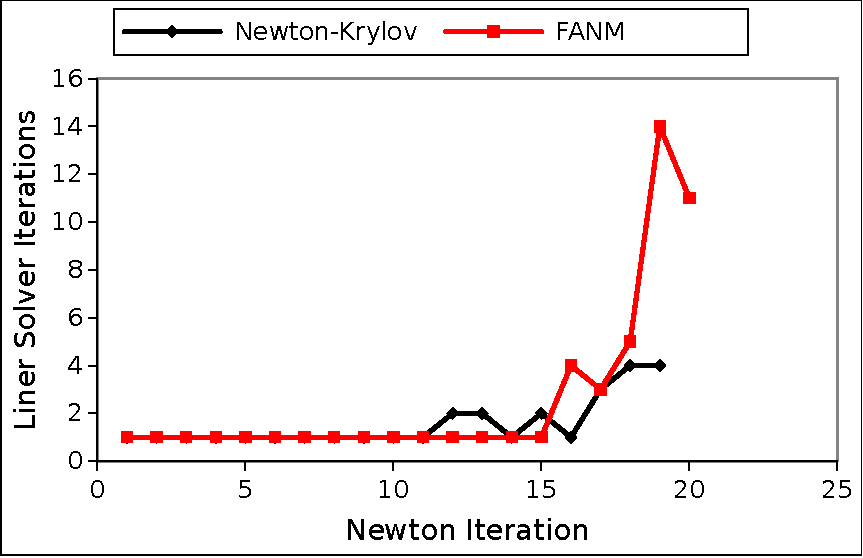
\includegraphics[width=6in]{chapters/nonlinear_problem/step_re500_iters.pdf}
  \end{center}
  \caption{\textbf{Backward facing step linear solver iterations as a
      function of Newton iteration for the 500 Reynolds number case.}
    \textit{More MCSA iterations were required to converge the linear
      models at later Newton iterations due to ill-conditioning of the
      Jacobian matrices.}}
  \label{fig:step_re500_iters}
\end{figure}

\begin{figure}[t!]
  \begin{center}
    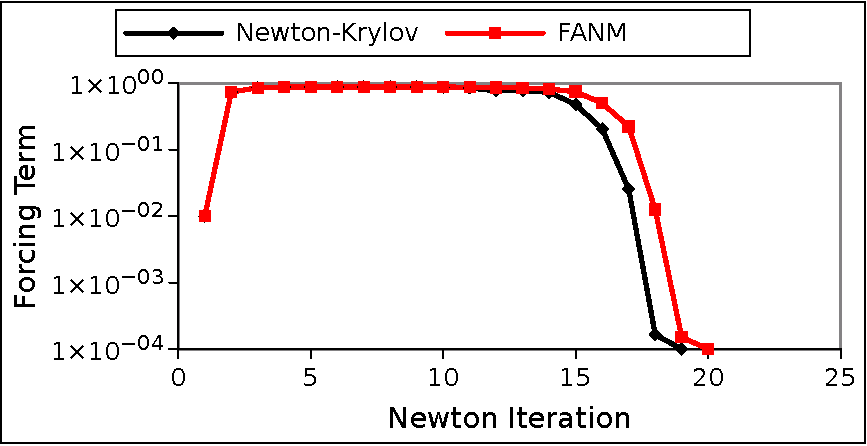
\includegraphics[width=6in]{chapters/nonlinear_problem/step_re500_forcing.pdf}
  \end{center}
  \caption{\textbf{Backward facing step forcing terms as a function of
      Newton iteration for the 500 Reynolds number case.} \textit{More
      MCSA iterations were required to converge the linear models at
      later Newton iterations due to ill-conditioning of the Jacobian
      matrices.}}
  \label{fig:step_re500_forcing}
\end{figure}

The ill-conditioning of the 500 Reynolds number case is also apparent
in the timing data given in
Table~\ref{tab:step_speedup_comparison}. For the first two cases, we
see qualitatively similar speedup values for the Newton-Krylov solver
relative to the observations for the first two benchmark problems of
O(100). However, we expect the ill-conditioning to cause the Monte
Carlo histories in the MCSA solver to have longer random walk lengths
based on our MCSA breakdown analysis in the previous chapter. In
addition, we observed that the linear model required many more MCSA
iterations to converge. These longer random walks and more iterations
manifest themselves in the longer CPU time values and therefore the
larger Newton Krylov speedup value of O(1,000) for the 500 Reynolds
number case.

\begin{table}[h!]
  \begin{center}
    \begin{tabular}{cc}\hline\hline
      \multicolumn{1}{c}{Reynolds Number}& 
      \multicolumn{1}{c}{Newton-Krylov Speedup}\\
      \hline
      200 & 400 \\
      300 & 593 \\
      400 & 825 \\
      500 & 1057 \\
      %%
      \hline\hline
    \end{tabular}
  \end{center}
  \caption{\textbf{Backward facing step Newton-Krylov speedup
      over FANM method.} \textit{Speedup values are rounded to the
      nearest integer. The results presented here were obtained from
      the benchmark verification calculations.}}
  \label{tab:step_speedup_comparison}
\end{table}


\subsection{Overall Performance Comparison}
\label{subsec:nonlinear_overall_comparison}

As a final overall comparison, we tabulate the results from the
benchmark calculations over the three performance metrics: nonlinear
iterations, linear iterations, and CPU
time. Tables~\ref{tab:benchmark_nonlinear_comparison},
\ref{tab:benchmark_linear_comparison}, and
\ref{tab:benchmark_time_comparison} give the results. In these tables,
the calculations that produced the best performing results are
tallied. In the case of a tie, both are tallied. Looking at the
tabulated results, we see marginally better performance for FANM in
terms of nonlinear iterations with 1 extra case outperforming the
Newton-Krylov method. As observed for each benchmark, the timing
results were always in favor of the Newton-Krylov method due to the
effects of the explicit preconditioning strategy.

For the total linear solver iterations given in
Table~\ref{tab:benchmark_linear_comparison}, the difference is more
dramatic with FANM converging the nonlinear residual in fewer linear
solver iterations for twice as many cases as the Newton-Krylov method,
keeping in mind that for all cases both GMRES and MCSA were
preconditioned with identical multigrid parameters using the same
multigrid preconditioning library. This shows that when properly
preconditioned, we can expect performance improvements in terms of
total linear solver iterations required to converge the nonlinear
residual. With future optimization of MCSA implementations, this may
also mean improved time to solution for FANM when compared to
Newton-Krylov methods.

\begin{table}[h!]
  \begin{center}
    \begin{tabular}{lcc}\hline\hline
      \multicolumn{1}{l}{Benchmark}& 
      \multicolumn{1}{c}{Newton-Krylov}&
      \multicolumn{1}{c}{FANM}\\
      \hline
      Convection, Ra=\sn{1}{3} & $\times$ & $\times$ \\
      Convection, Ra=\sn{1}{4} & $\times$ & $\times$ \\
      Convection, Ra=\sn{1}{5} & $\times$ & \\
      Convection, Ra=\sn{1}{6} & $\times$ & $\times$ \\
      Lid Driven, Re=100 & $\times$ & $\times$ \\
      Lid Driven, Re=300 & $\times$ & $\times$ \\
      Lid Driven, Re=500 & $\times$ & $\times$ \\
      Lid Driven, Re=700 & & $\times$ \\
      Backward Step, Re=200 & & $\times$ \\
      Backward Step, Re=300 & & $\times$ \\
      Backward Step, Re=400 & $\times$ & $\times$ \\
      Backward Step, Re=500 & $\times$ & \\
      %%
      \hline\hline
    \end{tabular}
  \end{center}
  \caption{\textbf{Navier-Stokes benchmark comparison for nonlinear
      iterations.} \textit{Over all benchmarks, FANM performed better
      in terms of nonlinear iterations for 1 more case than the
      Newton-Krylov method.}}
  \label{tab:benchmark_nonlinear_comparison}
\end{table}

\begin{table}[h!]
  \begin{center}
    \begin{tabular}{lcc}\hline\hline
      \multicolumn{1}{l}{Benchmark}& 
      \multicolumn{1}{c}{Newton-Krylov}&
      \multicolumn{1}{c}{FANM}\\
      \hline
      Convection, Ra=\sn{1}{3} & & $\times$ \\
      Convection, Ra=\sn{1}{4} & & $\times$ \\
      Convection, Ra=\sn{1}{5} & & $\times$ \\
      Convection, Ra=\sn{1}{6} & & $\times$ \\
      Lid Driven, Re=100 & $\times$ & \\
      Lid Driven, Re=300 & $\times$ & \\
      Lid Driven, Re=500 & $\times$ & \\
      Lid Driven, Re=700 & & $\times$ \\
      Backward Step, Re=200 & & $\times$ \\
      Backward Step, Re=300 & & $\times$ \\
      Backward Step, Re=400 & & $\times$ \\
      Backward Step, Re=500 & $\times$ & \\
      %%
      \hline\hline
    \end{tabular}
  \end{center}
  \caption{\textbf{Navier-Stokes benchmark comparison for total linear
      solver iterations.} \textit{Over all benchmarks, FANM performed
      better in terms of linear solver iterations for twice as many
      cases as the Newton-Krylov method.}}
  \label{tab:benchmark_linear_comparison}
\end{table}

\begin{table}[h!]
  \begin{center}
    \begin{tabular}{lcc}\hline\hline
      \multicolumn{1}{l}{Benchmark}& 
      \multicolumn{1}{c}{Newton-Krylov}&
      \multicolumn{1}{c}{FANM}\\
      \hline
      Convection, Ra=\sn{1}{3} & $\times$ & \\
      Convection, Ra=\sn{1}{4} & $\times$ & \\
      Convection, Ra=\sn{1}{5} & $\times$ & \\
      Convection, Ra=\sn{1}{6} & $\times$ & \\
      Lid Driven, Re=100 & $\times$ & \\
      Lid Driven, Re=300 & $\times$ & \\
      Lid Driven, Re=500 & $\times$ & \\
      Lid Driven, Re=700 & $\times$ & \\
      Backward Step, Re=200 & $\times$ & \\
      Backward Step, Re=300 & $\times$ & \\
      Backward Step, Re=400 & $\times$ & \\
      Backward Step, Re=500 & $\times$ & \\
      %%
      \hline\hline
    \end{tabular}
  \end{center}
  \caption{\textbf{Navier-Stokes benchmark comparison for CPU time.}
    \textit{For all benchmarks the explicit MCSA preconditioning
      strategy caused significantly larger CPU times for FANM when
      compared to the Newton-Krylov solutions.}}
  \label{tab:benchmark_time_comparison}
\end{table}

%%---------------------------------------------------------------------------%%
\section{Summary\ }
\label{sec:nonlinear_summary}

In this chapter we have developed and explored Monte Carlo Synthetic
Acceleration methods in the context of solutions to the Navier-Stokes
equations. The following are the significant observations, findings,
and contributions.

\begin{itemize}
\item Forward-Automated Newton-MCSA (FANM), a new inexact Newton
  method leveraging Monte Carlo Synthetic Acceleration, has been
  developed
\item The FANM method has been incorporated into the Drekar
  multiphysics production code base developed at Sandia National
  Laboratories
\item The FANM method has been verified to produce the same solutions
  as a production Newton-Krylov method for three difficult benchmark
  problems for the Navier-Stokes equations in different flow regimes
  and geometries
\item The FANM method has better iterative performance than the
  Newton-Krylov method for convection dominated problems, converging
  in fewer linear solver iterations with the same preconditioning for
  high and low Rayleigh numbers
\item The Newton-Krylov method has better iterative performance than
  the FANM method for flow dominated by inertial forces, converging in
  fewer linear solver iterations with the same preconditioning for
  high Reynolds numbers
\item Using more Monte Carlo histories at every FANM iteration was
  observed to reduce the number nonlinear iterations required to
  converge the lid-driven cavity problem at high Reynolds numbers
\item The spectral radius convergence restriction on MCSA was observed
  to be a significant hindrance by preventing solutions to forced flow
  problems at high Reynolds numbers
\item Explicit algebraic preconditioning used to overcome the spectral
  radius restriction of MCSA creates FANM run times
  $O(100)$-$O(1,000)$ slower than the Newton-Krylov solver
\end{itemize}
